\usetikzlibrary{positioning, shapes.geometric, fit, arrows.meta, patterns}
\usetikzlibrary{overlay-beamer-styles}
\begin{frame}
    \frametitle{Language Models}
    \begin{center}
        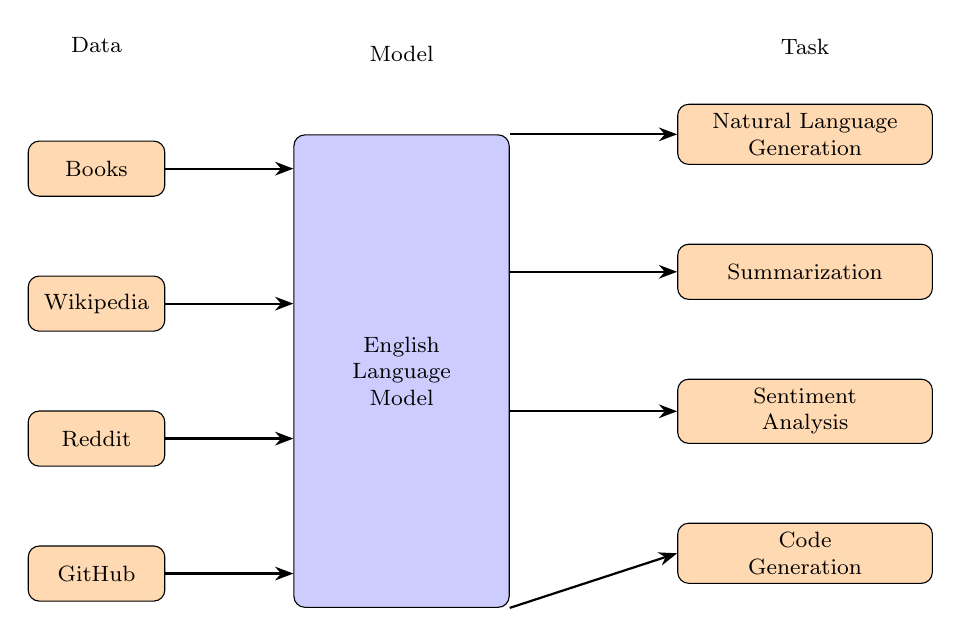
\begin{tikzpicture}[
            node distance=.7cm and 1.5cm,
            align=center,
            rounded corners,
            every node/.style={font=\footnotesize},
            input/.style={draw, fill=orange!30, text width=1.5cm, minimum height=0.7cm},
            model/.style={draw, fill=blue!20, text width=2.5cm, minimum height=6cm, align=center}, % Increased height
            % output/.style={text width=3cm, minimum height=0.8cm},
            output/.style={draw, fill=orange!30, text width=3cm, minimum height=0.7cm},
            arrow/.style={-Stealth, thick}
        ]



        % Input nodes (vertically aligned with equal spacing)
        \node[input, visible on=<2->] (books) {Books};
        \node[input, below=1cm of books, visible on=<2->] (wikipedia) {Wikipedia};
        \node[input, below=1cm of wikipedia, visible on=<2->] (reddit) {Reddit};
        \node[input, below=1cm of reddit, visible on=<2->] (github) {GitHub};

        % Model node (with taller height)
        \node[model, right=3cm of wikipedia.south east, yshift=-.5cm, anchor=center, visible on=<1->] (model) {English\\ Language\\ Model};

        % Output nodes (vertically aligned with equal spacing)
        \node[output, right=3.5cm of model.north, visible on=<3->] (nlg) {Natural Language\\ Generation};
        \node[output, below=1cm of nlg, visible on=<3->] (summ) {Summarization};
        \node[output, below=1cm of summ, visible on=<3->] (sentiment) {Sentiment\\ Analysis};
        \node[output, below=1cm of sentiment, visible on=<3->] (codegen) {Code\\ Generation};

                % Headings for sections
        \node[above=.5cm of books,  yshift=.5cm, visible on=<2->] {Data}; % Above inputs
        \node[above=.5cm of model, yshift=.3cm, visible on=<1->] {Model}; % Above model
        \node[above=.5cm of nlg, visible on=<3->] {Task}; % Above outputs

        % Arrows from inputs to model
        \draw[arrow, visible on=<2->] (books.east) -- (model.west |- books.east);
        \draw[arrow, visible on=<2->] (wikipedia.east) -- (model.west |- wikipedia.east);
        \draw[arrow, visible on=<2->] (reddit.east) -- (model.west |- reddit.east);
        \draw[arrow, visible on=<2->] (github.east) -- (model.west |- github.east);

        % Arrows from model to outputs
        \draw[arrow, visible on=<3->] (model.north east) -- (nlg.west);
        \draw[arrow, visible on=<3->] (model.east |- summ.west) -- (summ.west);
        \draw[arrow, visible on=<3->] (model.east |- sentiment.west) -- (sentiment.west);
        \draw[arrow, visible on=<3->] (model.south east) -- (codegen.west);

        \end{tikzpicture}
    \end{center}
\end{frame}

